\documentclass[12pt, aspectratio=43]{beamer} 

%%%%%%%%%%%%%%%%%%%%%%%%%%%%%%%%%%%%%%%%%
% 模板資訊：
% 模板名稱：Beamer
% 版本：1.0 (2023.07.09)
% 修改者：Ernie
% 編譯器：XeLaTeX
%
% 原始模板的資訊：
% 模板名稱：Beamer Presentation
% 作者：Vel (vel@latextemplates.com)
% 編譯器：XeLaTeX
% 授權：CC BY-NC-SA 4.0 (https://creativecommons.org/licenses/by-nc-sa/4.0/)
% 下載連結：https://www.LaTeXTemplates.com
%
% 製作本模板之目的：
% 為了讓 LaTeX 初學者能夠輕鬆地完成專業的學術簡報，因此我針對 Vel 製作的模板做了大幅度的修改及附上清楚明瞭的註解。
%
% 如果您有任何問題，可以透過 Email 聯繫我們：stateconlab@gmail.com
% 
% p.s. 也別忘了關注我們的 YouTube、IG 和 Medium 喔！
% 1. YouTube：https://www.youtube.com/@StatEconLab
% 2. IG：https://www.instagram.com/stateconlab
% 3. Mediun：https://medium.com/@stateconlab
%%%%%%%%%%%%%%%%%%%%%%%%%%%%%%%%%%%%%%%%%

%----------------------------------------------------------------------------------------
%	封包與文檔配置
%----------------------------------------------------------------------------------------

% 自訂字體的封包
\usepackage{fontspec} 

%% 設定中文字體
\usepackage{xeCJK}
\setCJKmainfont[AutoFakeBold=3.5 , AutoFakeSlant=0.2]{cwTeXYen}
\XeTeXlinebreaklocale "zh"
\XeTeXlinebreakskip = 0pt plus 1pt

%% 設定英文字體
\usefonttheme{serif} % 使用 serif 字體

% 自訂字體顏色的封包
\usepackage{color} 

%% 自訂顏色
\definecolor{Myblue}{RGB}{57,108,144}
\definecolor{Default_Blue}{RGB}{52,51,171}

% 數學工具及符號
\usepackage{mathtools, amsmath, amsfonts, amsthm, latexsym, amssymb} 

% 分別將數學符號間的間隔加大及加粗
\usepackage{newtxtext,newtxmath}

% 圖表自動編號的封包
\usepackage{caption} 

%% 設定自動編號
\setbeamertemplate{caption}[numbered]

%% 設定圖表編號及標籤的字體大小及字形
\captionsetup[figure]{font=small, labelfont=md}
\captionsetup[table]{font=small, labelfont=md}

% 導入圖形與表格的封包
\usepackage{graphicx}  % \scalebox{} 可用於將過大的表格縮小
\usepackage{booktabs}

% 排列多個子圖形的封包
\usepackage{subfigure} 

% 允許表格的一格能多列呈現的封包
\usepackage{multirow} 

% 可指定表格排版的封包
\usepackage{array}

% 翻轉表格的封包
\usepackage{lscape} 

% 序列標號
\usepackage{enumerate} 
\usetheme{Warsaw}
% 繪圖封包 (用於添加浮水印)
\usepackage{tikz}

% 引注參考資料
\usepackage{natbib}

% 註釋掉大部分的封包
\usepackage{comment}
\usepackage[most]{tcolorbox}
\usepackage{multicol}
\usepackage{xcolor}
% 設定中文的標籤
\renewcommand{\figurename}{圖} 
\renewcommand{\tablename}{表} 

% Colores
\definecolor{azul}{RGB}{20,119,180}
\definecolor{naranja}{RGB}{205,91,25}
\definecolor{fondo}{RGB}{250,249,247}
\definecolor{fondocaja}{RGB}{247,249,252}
\definecolor{texto}{RGB}{27,37,55}

% Estilo de las tarjetas
\newtcolorbox{modelbox}[1]{
    enhanced,
    colback=fondo,
    colframe=azul,
    boxrule=1.1pt,
    arc=3mm,
    left=3mm,
    right=3mm,
    top=3mm,
    bottom=3mm,
    height=6.4cm,
    valign=top,
    title={\textcolor{naranja}{\bfseries\small #1}},
    coltitle=naranja,
    attach boxed title to top left={
        xshift=2mm,
        yshift=-1mm
    },
    boxed title style={
        colback=fondo,
        boxrule=0pt
    }
}
%----------------------------------------------------------------------------------------
%	排版形式 (擇一，不選等同選擇默認的排版形式)
%----------------------------------------------------------------------------------------

\mode<presentation>{
%\usetheme{default}
%\usetheme{AnnArbor}
%\usetheme{Antibes}
%\usetheme{Bergen}
%\usetheme{Berkeley}
%\usetheme{Berlin}
%\usetheme{Boadilla}
%\usetheme{CambridgeUS}
%\usetheme{Copenhagen}
%\usetheme{Darmstadt}
%\usetheme{Dresden}
%\usetheme{Frankfurt}
%\usetheme{Goettingen}
%\usetheme{Hannover}
%\usetheme{Ilmenau}
%\usetheme{JuanLesPins}
%\usetheme{Luebeck}
\usetheme{Madrid}
%\usetheme{Malmoe}
%\usetheme{Marburg}
%\usetheme{Montpellier}
%\usetheme{PaloAlto}
%\usetheme{Pittsburgh}
%\usetheme{Rochester}
%\usetheme{Singapore}
%\usetheme{Szeged}
%\usetheme{Warsaw}

%----------------------------------------------------------------------------------------
%	外框形式 (擇一，不選等同選擇默認的外框形式)
%----------------------------------------------------------------------------------------

%\useoutertheme{default}
%\useoutertheme{infolines}
%\useoutertheme{miniframes}
%\useoutertheme{smoothbars}
%\useoutertheme{sidebar}
%\useoutertheme{split}
%\useoutertheme{shadow}
%\useoutertheme{tree}
%\useoutertheme{smoothtree}

%----------------------------------------------------------------------------------------
%	外框的自訂義調整 
%----------------------------------------------------------------------------------------

% 外框上緣的字 (fg) 為黑色，背景 (bg) 為白色。
%\setbeamercolor{section in head/foot}{fg=white, bg=black} 

% 外框上緣顯示的章節(section)頁數標籤是否關閉
%\setbeamertemplate{mini frames}{}   

% 調整外框形式的字體大小
\setbeamerfont{headline}{size=\scriptsize}
\setbeamerfont{footline}{size=\scriptsize}

% 取消右下方的跳轉工具列
\setbeamertemplate{navigation symbols}{} 

%% 自定義1：外框下緣僅出現名字及頁碼
%\setbeamertemplate{footline}
%{\leavevmode%
%\hbox{%
%\begin{beamercolorbox}[wd=0.5\paperwidth,ht=3ex,dp=1ex,leftskip=2ex]%
%{author in head/foot}%
%{\footnotesize\textbf{\insertshortauthor}}%
%\end{beamercolorbox}%
%\begin{beamercolorbox}[wd=0.5\paperwidth,ht=3ex,dp=1ex,right]%
%{author in head/foot}%
%\footnotesize \textbf{{\insertframenumber{} / \inserttotalframenumber\hspace*{2ex}}} %頁碼控制選項
%\end{beamercolorbox}%
%}}

%% 自定義2：清除外框下緣但僅出頁碼
%\setbeamertemplate{footline}[page number] 

%% 自定義3：清除外框下緣
%\setbeamertemplate{footline}[] 

%----------------------------------------------------------------------------------------
%	顏色主題 (擇一，不選等同選擇默認的顏色主題)
%----------------------------------------------------------------------------------------

\usecolortheme{default}
%\usecolortheme{albatross}
%\usecolortheme{beaver}
%\usecolortheme{beetle}
%\usecolortheme{crane}
%\usecolortheme{dolphin}
%\usecolortheme{dove}
%\usecolortheme{fly}
%\usecolortheme{lily}
%\usecolortheme{orchid}
%\usecolortheme{rose}
%\usecolortheme{seagull}
%\usecolortheme{seahorse}
%\usecolortheme{whale}
%\usecolortheme{wolverine}

%----------------------------------------------------------------------------------------
%	顏色主題的自訂義調整 
%----------------------------------------------------------------------------------------

% 全文的主題色 (可以特別針對報告對象或機構的代表色調整！)
\setbeamercolor{structure}{fg=Myblue} 

% 封面頁中標題區塊的底色及字體顏色
%\setbeamercolor{title}{bg=green, fg=black} 

% 各頁標題區塊的底色及字體顏色
%\setbeamercolor{frametitle}{bg=white,fg=black} 

% 全文的內文顏色
%\setbeamercolor{normal text}{fg=orange}

% 數學區塊的標題顏色 
%\setbeamercolor{block title}{bg=blue,fg=yellow} 

% 數學區塊的內文顏色 
%\setbeamercolor{block body}{bg=green,fg=red} 

% 警示文字的顏色
\setbeamercolor{alerted text}{fg=red} 

%----------------------------------------------------------------------------------------
%	enumerate 及 item 的形狀
%----------------------------------------------------------------------------------------

%\useinnertheme{rounded} % 圓球 (3D)
%\useinnertheme{circles} % 圓形 (2D)
%\useinnertheme{rectangles} % 方形
%\useinnertheme{triangle} % 三角形
%\useinnertheme{inmargin} % 插入邊沿
\setbeamertemplate{itemize items}[triangle]

%----------------------------------------------------------------------------------------
%	自訂 item 的顏色
%----------------------------------------------------------------------------------------

%\setbeamercolor{item projected}{bg=red}

%----------------------------------------------------------------------------------------
%	個人化的設置及細節調整
%----------------------------------------------------------------------------------------

% 設定頁面邊界
\setbeamersize{text margin left=0.6cm, text margin right=0.6cm}
\special{papersize=\the\paperwidth,\the\paperheight}
\providecommand{\tabularnewline}{\\}
}

%----------------------------------------------------------------------------------------
%	個人化的背景調控
%----------------------------------------------------------------------------------------

% 背景照片設置
%\setbeamertemplate{background}{
\includegraphics[height=\paperheight]{Fig/Background.png}}

% 浮水印設定
%\usebackgroundtemplate{%
%	\tikz[overlay, remember picture] % 讓 logo 能每頁都顯示
%	\node[opacity=0.3, below=-1.25cm, at=(current page.center)] % 調整透明度 (opacity) 及浮水印的位置
%	{
\includegraphics[scale = 0.14]{Fig/nthulogo.png}}; % 載入 logo 及調整大小
%	}



\usepackage[spanish, es-tabla]{babel}
\usepackage{ragged2e}

\begin{document}

\title[Proyecto Final]{\Large{\textbf{Imagen por Resonancia Magnética con Difusión}}} 

\institute[CIMAT Aguascalientes]{ \large Proyecto final \\
\large Laboratorio de resolución de problemas I}
\date[]{ 27 de noviembre de 2026}

\titlegraphic{
\includegraphics[width=2cm]{logo-cimat-ags.jpg}}

% Configuración para que la tabla de contenidos aparezca limpia al inicio de cada sección
\AtBeginSection[]{
  \begin{frame}<beamer>
    \frametitle{Contenido} % Cambiado de "Roteiro" a "Contenido"
    \tableofcontents[currentsection] % currentsubsection se quitó para que se vea más ordenado
  \end{frame}
}


\begin{frame}
	\titlepage 
\textit{}\end{frame}

\begin{frame}{\textbf{Contenido}}
	\tableofcontents 
\end{frame}

%--------------------------------------------------------------------------------------%
\section{Introducción}
\begin{frame}{Introducción}
\begin{multicols}{2}
    \begin{figure}
        \centering
        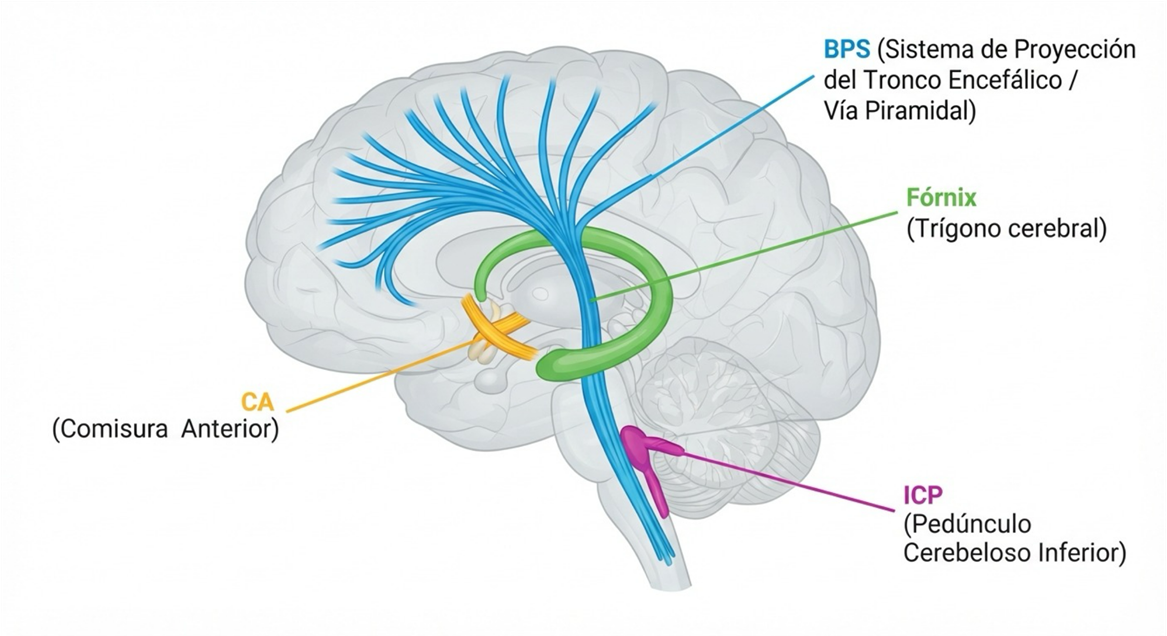
\includegraphics[width=1\linewidth]{image_cerebro.png}
        \caption{Haces de fibras nerviosas}
        \label{fig:placeholder}
    \end{figure}

    \begin{itemize}
        \item La tactografía dibuja las conexiones del cerebro con miles de curvas llamadas streamlines (hilos).
        \item Una gran parte de esos hilos parece real, pero no sigue ningún haz verdadero.
        %\item \huge{¿Como saber cuales conservar?.}
    \end{itemize}
\end{multicols}
\end{frame}

\begin{frame}{}
    \centering
    \huge{¿Como se determina cuáles streamlines se deben conservar?}
\end{frame}

\begin{frame}{Métodos de filtrado de tractogramas}
    %Los métodos de filtrado de tractogramas (tractogram filtering) son
    Comúnmente para determinar cuales streamlines conservar se utilizan técnicas que, a partir de un tractograma, asignan a cada streamline un peso, estimado a partir de la señal de difusión. \\
    %asignan a cada streamline un peso no negativo, estimado a partir de la señal de difusión. \\
    %, para evaluar qué tan bien se sostiene cada trayectoria con los datos medidos.

    \pause
    \vspace{0.5cm}
    {\large \textcolor{red}{Métodos}}:
    \begin{multicols}{3}
         \begin{itemize}
        \item \textbf{LiFE}%: ajusta los pesos directamente sobre la señal de difusión.
        \item \textbf{COMMIT}%: también ajusta sobre la señal, pero con un modelo de tres partes (dentro del axón, alrededor y agua libre).
        \item \textbf{SIFT2}%: ajusta los pesos para que la densidad de fibras coincida con la FOD.
    \end{itemize}
    \end{multicols}
\end{frame}

%\begin{frame}{ }
%\centering
   % \huge{¿Como hacerlo?}
%\end{frame}


\begin{frame}{Características de los métodos de filtrado}
\begin{center}
\begin{columns}[T]

\column{0.32\textwidth}

\textbf{LiFE}

\vspace{0.2cm}

\begin{itemize}
    \item Simula la señal de difusión generada por cada streamline y compara con la señal real.
    \item Conserva los streamlines que ayudan a explicar la señal.
\end{itemize}

\column{0.32\textwidth}

\textbf{COMMIT}

\vspace{0.2cm}

\begin{itemize}
    \item Estima la contribución individual de cada streamline a través de un modelo físico de difusión.
    \item Penaliza conexiones redundantes o poco útiles.
\end{itemize}

\column{0.32\textwidth}

\textbf{SIFT2}

\vspace{0.2cm}

\begin{itemize}
    \item Ajusta pesos dentro del tractograma en busca de coherencia con la densidad de fibras estimada.
    \item Rebalancea la importancia de cada streamline.
\end{itemize}

\end{columns}    
\end{center}
\end{frame}



%\begin{frame}{ }
%\centering
   % \huge{¿Como hacerlo?}
%\end{frame}

%--------------------------------------------------------------------------------------%
\section{Modelos de Aprendizaje automático}

\begin{frame}{}
\centering
    {\huge ¿Sirve más un modelo lineal o uno que pueda capturar relaciones no lineales entre los pesos?}\\
    
\end{frame}

\begin{frame}{Respondiendo a la pregunta}

\begin{multicols}{2}
    \justifying
    Para determinar si una combinación no lineal de los pesos generados puede identificar de forma más precisa los streamlines compatibles, se propone el uso de \textbf{modelos de aprendizaje automático}.

    \begin{figure}
    \centering
    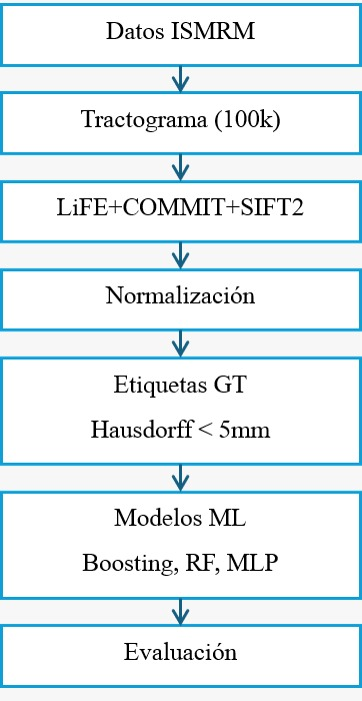
\includegraphics[height=0.6\textheight]{img_flujo.png}
    \caption{Flujo de trabajo}
    \label{fig:placeholder}
    \end{figure}
    
\end{multicols}
\end{frame}

\begin{frame}{Modelos de Aprendizaje automático}

    Aprenden patrones a partir de ejemplos para realizar predicciones. \\

    Se encargan de Clasificar y estimar un valor numérico. 
    \vspace{0.5cm}    \pause
    \begin{itemize}
        \item \textbf{Bosque aleatorio (RF)}.
        \item \textbf{Gradient boosting (GB)}.
        \item \textbf{Perceptron multicapa (MLP)}.
    \end{itemize}
\end{frame}


\begin{comment}
    \begin{frame}{Bosque aleatorio}
    Combina muchos árboles de decisión para producir una predicción conjunta. 
    %Varios árboles de decisión, cada uno entrenado con una muestra distinta de los hilos, y se promedian sus votos.

    \begin{itemize}
        \item 400 árboles de decisión. 
    \end{itemize}
\end{frame}

\begin{frame}{Gradient boosting}

    Construye modelos de forma secuencial, cada nuevo modelos intenta corregir errores anteriores. 
    %Árboles pequeños, uno tras otro. Cada uno corrige lo que el conjunto anterior todavía predice mal.
    
\end{frame}

\begin{frame}{MLP}
    \begin{itemize}
        \item  Red neruronal artificial que aprende ajustando los pesos de sus conexiones. 
        \item Se utilizaron  128 - 64 - 32 neuronas.
        
    \end{itemize}

\end{frame}
\end{comment}

\begin{frame}{Modelo 1: Random Forest}

\begin{block}{Modelo matemático}
\[
\boxed{
p(x)=\frac{1}{B}\sum_{b=1}^{B}T_b(x)
}
\]

\small
Donde $B$ es el número de árboles y $T_b(x)$
representa la probabilidad estimada por el árbol $b$.
\end{block}

\pause

\textbf{\textcolor{blue}{¿Cómo funciona?}}

\justifying
Construye múltiples árboles de decisión utilizando muestras aleatorias de los datos y subconjuntos de variables. La predicción final se obtiene \textbf{promediando las probabilidades de todos los árboles.}

\vspace{0.3cm}


\end{frame}


\begin{frame}{Random Forest: configuración}

\begin{columns}[T,onlytextwidth]

\begin{column}{0.48\textwidth}
\textbf{\textcolor{blue}{Hiperparámetros}}

\begin{itemize}
    \item Número de árboles: 400.
    \item \texttt{max\_features}: 0.5.
    \item \texttt{min\_samples\_leaf}:
    \begin{itemize}
        \item 20 con longitud.
        \item 100 sin longitud.
    \end{itemize}
    \item Búsqueda de hiperparámetros.
\end{itemize}
\end{column}

\begin{column}{0.48\textwidth}
\textbf{\textcolor{blue}{Variables utilizadas}}

\begin{itemize}
    \item Logaritmo de los pesos.
    \item Indicadores de presencia.
    \item Número de métodos que conservan el hilo.
    \item Longitud (variante adicional).
\end{itemize}
\end{column}

\end{columns}

\vspace{0.4cm}

\begin{block}{Entrenamiento}
Se reservó un 20\% de los datos para la búsqueda de hiperparámetros (tuning). Se seleccionó la configuración con mejor desempeño en validación para evitar sobreajuste.
\end{block}

\end{frame}


\begin{frame}{Modelo 2: Gradient Boosting}
\begin{block}{Modelo matemático}
\[
\boxed{
p(x)=\sigma\left(
F_0+\nu\sum_{m=1}^{M}h_m(x)
\right)
}
\]

\small
Donde $F_0$ es la predicción inicial, $\nu$ la tasa de aprendizaje,
$h_m(x)$ la contribución del árbol $m$ y $M$ el número de iteraciones.
\end{block}

\textbf{\textcolor{blue}{¿Cómo funciona?}}

\justifying
Construye árboles de decisión de manera secuencial. \textbf{Cada nuevo árbol busca corregir los errores del modelo acumulado,} mejorando progresivamente las predicciones.

\vspace{0.3cm}

%\begin{alertblock}{Función en el proyecto}
%Aprender patrones complejos mediante la construcción
%progresiva de árboles de decisión.
%\end{alertblock}

\end{frame}

\begin{frame}{Gradient Boosting: configuración}

\begin{columns}[T,onlytextwidth]

\begin{column}{0.48\textwidth}
\textbf{\textcolor{blue}{Hiperparámetros}}

\begin{itemize}
    %\item Implementación: HistGradientBoostingClassifier.
    \item Profundidad: 6.
    \item Tasa de aprendizaje:
    \begin{itemize}
        \item 0.05 o 0.1 con longitud.
        \item 0.1 o 0.03 sin longitud.
    \end{itemize}
    \item Regularización.
    \item Mínimo de muestras por hoja: 50.
\end{itemize}
\end{column}

\begin{column}{0.48\textwidth}
\textbf{\textcolor{blue}{Entrenamiento}}

\begin{itemize}
    \item Máximo: 1000 iteraciones.
    \item Validación interna: 15\%.
    \item Detención temprana.
    \item Paciencia: 20 iteraciones.
    \item Búsqueda de hiperparámetros.
\end{itemize}
\end{column}
\end{columns}
\end{frame}

\begin{frame}{Modelo 3: MLP}

\begin{block}{Modelo matemático}

\[
h_k=\operatorname{ReLU}(W_kh_{k-1}+b_k)
\]

\[
\boxed{
p(x)=\sigma(w^Th_3+b)
}
\]

\small
La salida de la tercera capa oculta se transforma en una
probabilidad mediante la función sigmoide.

\end{block}

\textbf{\textcolor{blue}{¿Cómo funciona?}}

La red recibe las características de cada hilo y las procesa mediante tres capas ocultas. Cada capa aprende representaciones de la información para identificar patrones relacionados con la clasificación.
\end{frame}


\begin{frame}{MLP: arquitectura y entrenamiento}

\begin{center}

\begin{block}{Arquitectura de la red neuronal}
\[
\boxed{
\text{Entrada}
\longrightarrow 128
\longrightarrow 64
\longrightarrow 32
\longrightarrow \text{Salida}
}
\]
\end{block}

\end{center}

\begin{columns}[T,onlytextwidth]

\begin{column}{0.48\textwidth}
\textbf{\textcolor{blue}{Arquitectura}}

\begin{itemize}
    \item Tres capas ocultas.
    \item 128, 64 y 32 neuronas.
    \item Activación ReLU.
    %\item Batch Normalization.
    \item Dropout: 0.15 y 0.10.
\end{itemize}
\end{column}

\begin{column}{0.48\textwidth}
\textbf{\textcolor{blue}{Entrenamiento}}

\begin{itemize}
    \item Optimizador: AdamW.
    \item Tamaño de lote: 1024.
    \item Máximo: 200 veces.
    \item Paciencia: 15 veces.
    \item Cinco semillas.
    \item Promedio de cinco entrenamientos.
\end{itemize}
\end{column}

\end{columns}

%\vspace{0.3cm}

%\begin{block}{Variables adicionales}
%Rangos percentiles de los pesos e interacciones entre
%peso y longitud, además de las características comunes.
%\end{block}
\end{frame}

\begin{frame}{Entrenamiento de los modelos}
    Se utilizó un procedimiento de intercambio de mitades para garantizar que cada hilo fuera evaluado por un modelo que no lo hubiera utilizado durante su entrenamiento.\\
    \begin{figure}
        \centering
        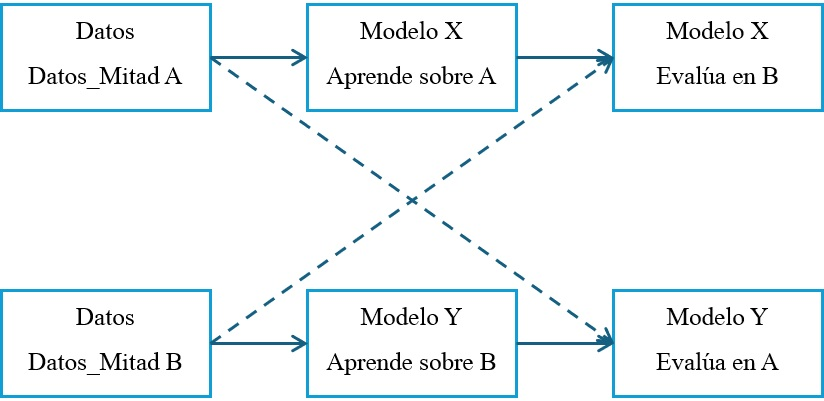
\includegraphics[width=.75\linewidth]{flujo_mitades.jpeg}
        \caption{Entrenamieto por mitades}
        \label{fig:placeholder}
    \end{figure}
\end{frame}
%--------------------------------------------------------------------------------------%

\section{Resultados}
\begin{frame}{Métrica de Hausdorff}
\begin{center}
\resizebox{0.98\textwidth}{!}{%
\begin{tabular}{||c c c c c c c c c||} 
 \hline
 hilo & longitud-mm & SIFT2 & COMMIT & LiFE & COMMIT2 & hd-min-mm &etiqueta-5mm & conjunto \\ [0.5ex] 
 \hline\hline
 0 & 67.3951 & 0.81755788 & 0 & 0.0022243596 & 0 & 0 & & entrenamiento \\ 
 \hline
 1 & 107.186 & 0.28476988 & 0 & 0 & 0 & 0 & & entrenamiento \\
 \hline
 2 & 24.8161 & 2.1176974 & 0.00737445 & 0.00019227226 & 0 & 0 & & prueba \\
 \hline
 3 & 102.284 & 0.81957053 & 0 & 0.0029736649 & 0.00119002 & 4.6321603 & 1 & prueba \\
 \hline
\end{tabular}%
}
\end{center}
donde:
\begin{itemize}
    %\item \textit{hilo:} es un streamline. 
    %\item \textit{longitud-mm:} es el largo del hilo en mm. 
    %\item \textit{SIFT2, COMMIT, LiFE,COMMIT2:} los pesos que cada método asignó al hilo. 
    \item \textit{hd-min-mm:} distancia de Hausdorff al Ground Truth en mm.  
    \item \textit{etiqueta-5mm:} vale  1 (verdadero) si hd-min-mm < 5 y 0 (falso) en otro caso.  
    \item \textit{conjunto:} si corresponde al conjunto de prueba o entrenamiento. 
\end{itemize}
\end{frame}

\begin{frame}{¿Qué obtuvimos?}
\begin{itemize}
    \item El $33 \% $ de los hilos son verdaderos. 
    \item El AUC por hilo de cada método es $0.426$ (SIFT2),
$0.449$ (COMMIT), $0.601$ (LiFE), $0.634$ (COMMIT2).
\item Hay muchos ceros en los pesos. 
\end{itemize}
    
\end{frame}

\begin{comment}
\begin{frame}{Decisión sobre las variables}
Se consideran: \textit{SIFT2}, \textit{COMMIT}, \textit{LiFE}, \textit{COMMIT2}, \textit{longitud-mm},  pues es la información que se conoce de un hilo sin el ground truth. 

\vspace{1 cm}

Se excluyen: \textit{hd-min-mm}, \textit{etiqueta-5mm}, pues dependen del GT y \textit{hilo}, \textit{conjunto} sólo son identificadores, no describen los hilos. 
\end{frame}    
\end{comment}

\begin{frame}{Resultado de los modelos}
    \begin{center}
\begin{tabular}{||c c c c c ||} 
 \hline
 Modelo & Longitud & AUC & 10000  &50000 \\ [0.5ex] 
 \hline\hline
 logística  & no & 0.688 & $46.5\%$  & $46 \% $ \\ 
 \hline
logística & si & 0.699 & $45 \%$  & $46.7 \%$ \\
\hline
boosting (sin ajustar) & no & 0.725 & $63.4 \%$ & $47.4 \%$ \\
\hline
 boosting (sin ajustar) & si & 0.793 & $69.8 \%$  & $52.5 \%$ \\
 \hline
 boosting (ajustado) & no & 0.727 & $63.8 \%$ & $47.5 \%$ \\
 \hline
 \textbf{boosting} (ajustado) & si & 0.798 & $70.4 \%$ & $52.7 \%$ \\
 \hline
  \textbf{bosque ajustado} & si & 0.799 & $71.4 \%$ & $53 \%$ \\
  \hline
  \textbf{MLP} (ajustado) & si & 0.799 & $70.8 \%$ & $53 \%$ \\
 \hline
\end{tabular}
\caption{AUC y porcentaje de hilos verdaderos entre los 10 000 y 50 000 de mayor puntaje.}
    \label{tab:ejemplo}
\end{center}
\end{frame}

\begin{frame}{Ajuste de los modelos}
\begin{center}
\renewcommand{\arraystretch}{1.6}
\begin{tabular}{@{}l>{\raggedright\arraybackslash}p{3.2cm}>{\raggedright\arraybackslash}p{5.2cm}@{}}
\toprule
\textbf{Modelo} & \textbf{Versión base} & \textbf{Versión ajustada}\\
\midrule
\textbf{Bosque}   & 200 árboles             & 400 árboles + búsqueda de hiperparámetros\\
\textbf{Boosting} & 300 árboles, prof.\ 4   & Parada temprana + búsqueda de profundidad y tasa\\
\textbf{MLP}      & Red 64--32, 3 semillas  & Red 128--64--32, \textit{dropout}, 5 semillas\\
\bottomrule
\end{tabular}
\end{center}

\vspace{0.6cm}
\centering
La búsqueda se hizo solo con la mitad de \textbf{entrenamiento}.\\
La mitad de prueba nunca interviene.
\end{frame}
%--------------------------------------------------------------------------------------%
\section{Conclusiones}

\begin{frame}{Conclusiones}
    \begin{enumerate}
        \item Sirve más un modelo no lineal: el bosque aleatorio, el \textit{gradient boosting} y el MLP alcanzan un AUC de $0.80$, frente a $0.70$ del modelo lineal (regresión logística).

        \item La combinación de los métodos de filtrado mediante modelos de aprendizaje automático supera el desempeño de cada método por separado (AUC $\approx 0.80$ frente a $0.43$--$0.60$ de \textit{SIFT2}, \textit{COMMIT} y \textit{LiFE}).

        \item La longitud del hilo mejora la clasificación solo en los modelos no lineales: en el \textit{gradient boosting} el AUC sube de $0.727$ a $0.798$, mientras que en la regresión logística apenas pasa de $0.688$ a $0.699$.

        \item Los tres modelos ajustados presentan un desempeño prácticamente igual (AUC $0.798$--$0.799$).
        
    \end{enumerate}
\end{frame}


\begin{frame}{}
\centering
    \textbf{\huge Gracias por su atención }
\end{frame}

\begin{frame}{}
    \begin{figure}
        \centering
        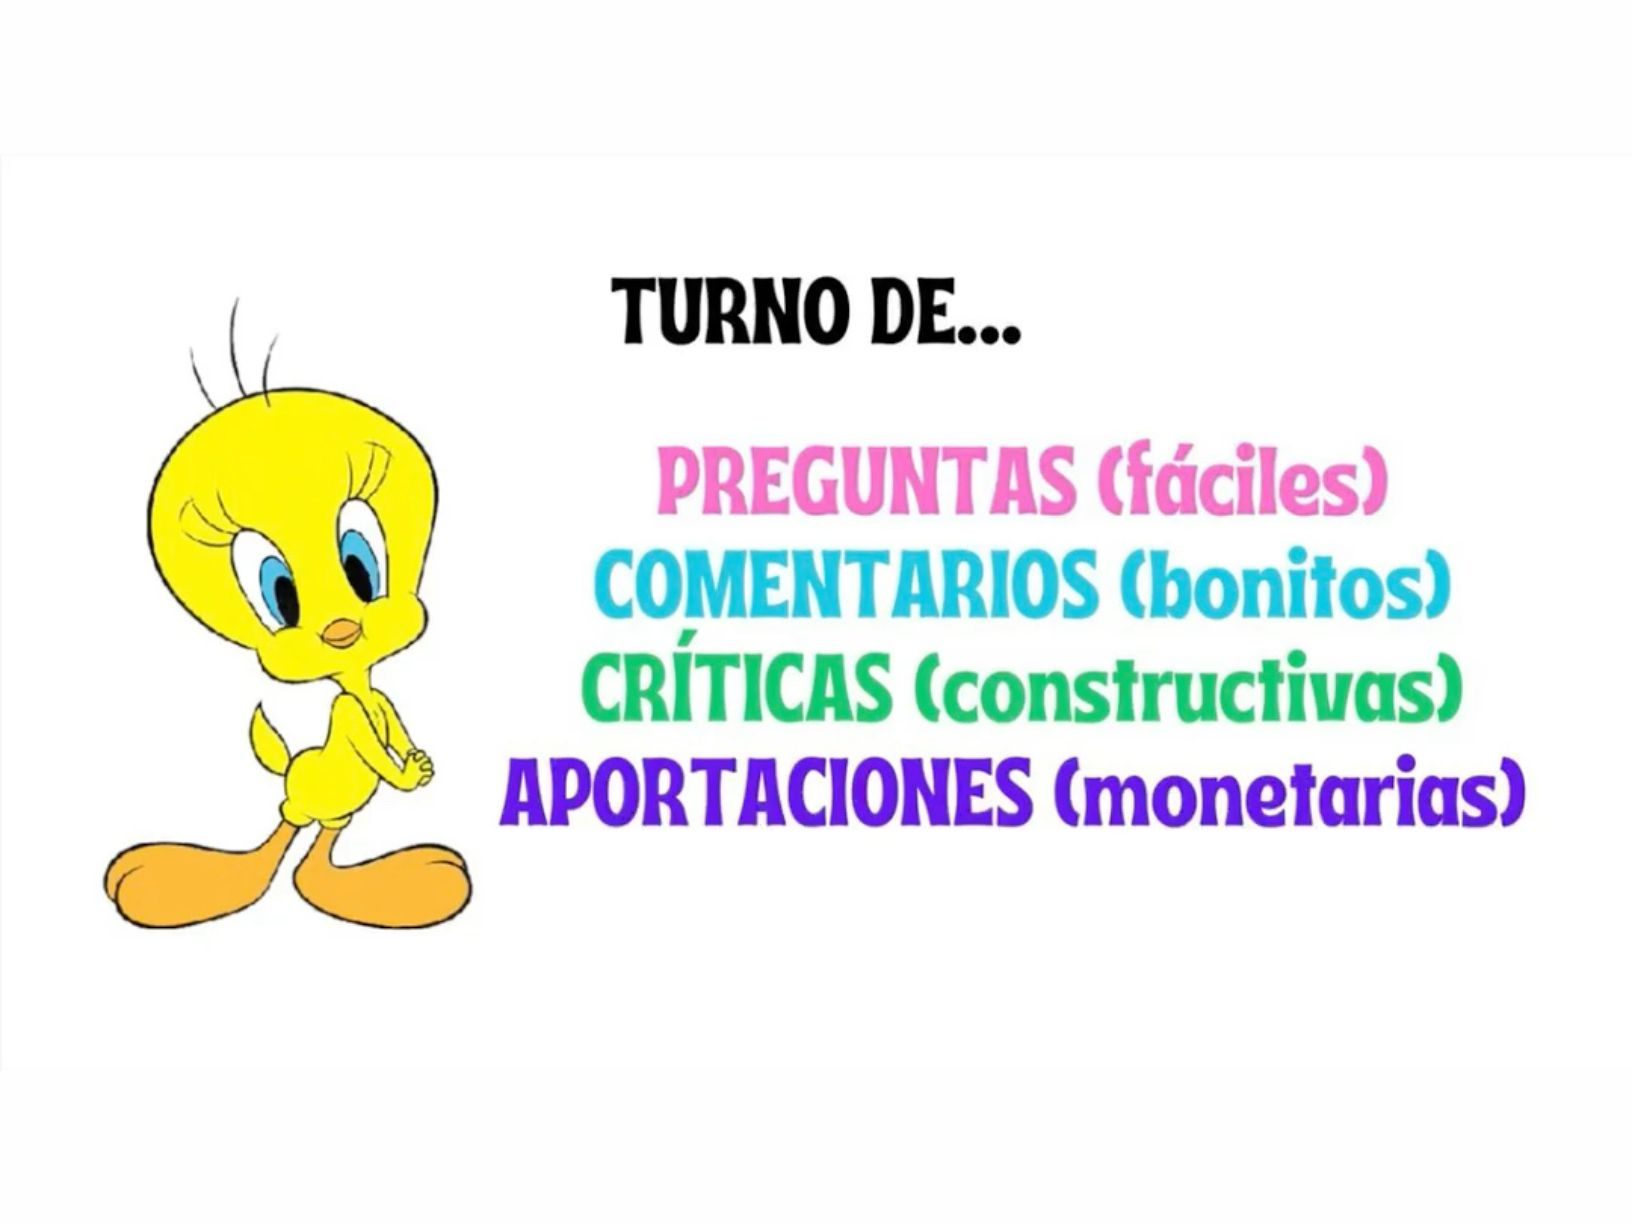
\includegraphics[width=0.8\linewidth]{aa06b4308b1a43aecadca6c9121b5312.jpg}
        \label{fig:placeholder}
    \end{figure}
\end{frame}
\end{document}